% RL and Policy Search intro ( introducing helicopter too)
Reinforcement learning is concerned with how agents should take actions in an environment such that the reward is maximized. The policy of an agent (it's behavior) is learned by repeatedly acting in an environment and receiving a reward for each action given the state of the environment. One class of Reinforcement learning is \textit{direct policy search}, a family of methods that directly searches the policy space in order to find the optimal policy. \\
One of the areas where policy search methods have proven to be useful is in control problems. However, further improvements upon existing methods are however needed for efficiently discovering highly effective policies for complex tasks. An example of such a problem is the helicopter control problem, %ref toevoegen 
a problem where a simulation model exists to evaluate policies. Evolutionary algorithms have proven to perform reasonably well \cite{koppejan2011neuroevolutionary}, but suffer from the high sample complexity as simulations are computationally costly. Another challenge in this problem is that the performance of a policy is determined largely by infrequent events, on which performance is hardly ever evaluated.

% Issue no controllable rare events are tested: solution = co-evolutionary approach
Focusing on controllable rare events (defined in more detail in section \ref{background}) for policy search would improve efficiency significantly. In order to be able to focus on particular events we define an outcome $z$, which specifies the result of every stochastic transition that could occur in a given episode. Thus a given policy $\pi$ and outcome $z$, an episode is deterministic. Instead of wasting random trials on non-informative $z$, this project leverages co-evolutionary principles to evolve both policies $\pi$ as well as outcomes $z$. The main idea is to improve the evolution process of the population policies by evaluating them on a population of outcomes, which are evolved specially to test the policies.

% Issue evolutionary forgetting
A known issue in co-evolution is co-evolutionary forgetting \cite{forgetting}: policies that excel against new predictors may perform poorly against older ones. This comes from the fact that the new policies only get tested against these new outcomes, but not the older ones. By maintaining a posterior belief, in the form of a gaussian process, over the fitness of policy-outcome pairs previous found results can be remembered. 

\begin{figure}[ht]
  \centering
  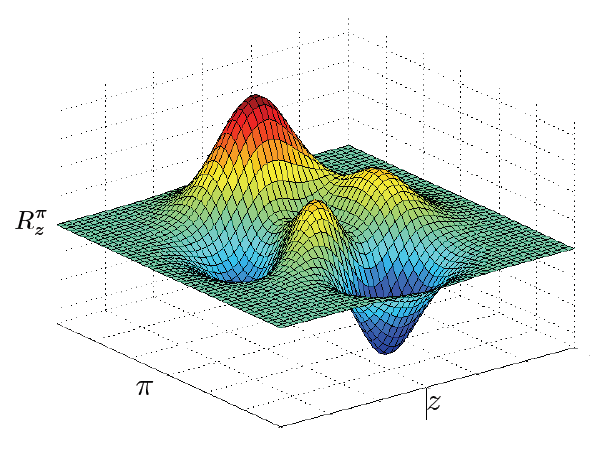
\includegraphics[scale=0.5]{images/fitness-landscape.png}
  \caption{Extended fitness landscape, where the reward is plotted given a policy $\pi$ and outcome $z$}\label{fitnesslandscape}
\end{figure}

% Approach in general
<<<<<<< HEAD
This posterior belief, as shown in figure \ref{fitnesslandscape}, attempts to map policy-outcome pairs to a reward. The challenge in this approach is to select appropriate pairs to evaluate and used to fit, called the acquisition function. Given a appropriate acquisition function, new data points are added to the landscape until a stop condition is met. Afterwards the best policy is extracted from the Gaussian process. We call this method \textbf{G}aussian \textbf{P}rocess - \textbf{C}o-\textbf{E}volutionary \textbf{P}olicy \textbf{S}earch, or \textbf{GP-CEPS} for short. \\


% outro: outline rest of paper
In the next section (\ref{background}) the background is provided, followed by related work (section \ref{related}). In section \ref{contrib} our approach is discussed in more detail, after which the experiments (\ref{experiments}) are shown. Lastly the results are discussed (section \ref{discussion}) and concluded (\ref{conclusion}).
>>>>>>> ad62e6aee5975c94878c0577d376e777f67e5877


